\FloatBarrier

Um die Oberflächengüte des Rheniumkristalls zu analysieren, wurde die Oberfläche zunächst mit LEED
untersucht. Zuvor wurde die Probe bei einer Hochspannung von \SI{700}{V} und einem Strom
von \SI{150}{mA} zwischen Filament und Probe geflasht. Dies entspricht etwa einer Temperatur von
etwa \SI{1000}{K}.
\\
Rhenium hat eine hcp-Kristallstrukur, daher erwartet man auch als Beugungsmuster an der Oberfläche
eine hexagonale Periodizität. Zwar ist das LEED-Beugungsbild eine direkte Abbildung des reziproken
Raums, nicht des Realraums, doch ist das reziproke Gitter einer hcp-Struktur wiederum eine
hcp-Struktur.
\\
Alle hier abgebildeten LEED-Bilder entstanden durch Abfotografieren des Phosphorschirms der
LEED-Vorrichtung. Zu Beobachten sind normalerweise helle Punkte auf dunklem Hintergrund; zur
besseren Darstellung wurden hier die Farben invertiert.
\\
Bei einer Elektronenergie von \SI{208}{eV} ergaben sich Beugungsmuster wie in Abb. \ref{rekristall}.
Es zeigte sich, dass die Oberfläche keine homogene Güte besitzt. In den äußeren Bereichen des
Kristalls ist die Struktur gekennzeichnet durch scharfe Spots und ein hexagonales
Muster, was auf eine periodische, planare Oberfläche hinweist. In der Mitte des Kristalls jedoch
besitzt die Oberfläche eine unregelmäßige Struktur; die Hauptspots heben sich kaum von den ungleich
verteilen Spots der Überstruktur ab.

\begin{figure}[htbp]
	\begin{minipage}[b]{0.5\textwidth}
	
		\begin{overpic}[width=\textwidth]{LEED-Bilder/bearbeitet/unbedampft_E207}
        	\put(1,71){a)}
  		\end{overpic}
	\end{minipage}
	\hfill
	\begin{minipage}[b]{0.5\textwidth}
		\begin{overpic}[width=\textwidth]{LEED-Bilder/bearbeitet/unbedampft_E207_MitteKristall.jpg}
        	\put(1,71){b)}
  		\end{overpic}
	\end{minipage}
	\caption{\textit{a) Der Re-Kristall mit scharfen Spots und hexagonaler Struktur aus dem
	Randbereich der Probe.
	b) Die Re-Oberfläche in der Mitte der Probe mit Verschmutzung, zu erkennen an der Überstruktur und
	den schwächeren Hauptspots.
	Beide Beugungsmuster sind bei einer Elektronenenergie von \SI{208}{eV} entstanden.}}
	\label{rekristall} 
\end{figure}
 

\begin{figure}[H]
		\captionsetup{name=Abb.}
	\begin{minipage}[b]{0.5\textwidth} 
		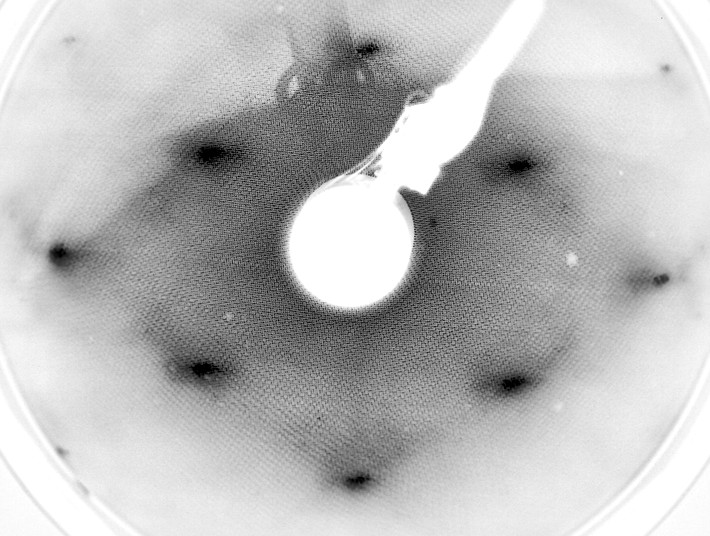
\includegraphics[width=\textwidth]{LEED-Bilder/bearbeitet/unbedampft_E207}
		\caption{\textit{Re-Oberfläche}}
		\label{0ML} 
	\end{minipage}
	\hfill
	\begin{minipage}[b]{0.5\textwidth}
		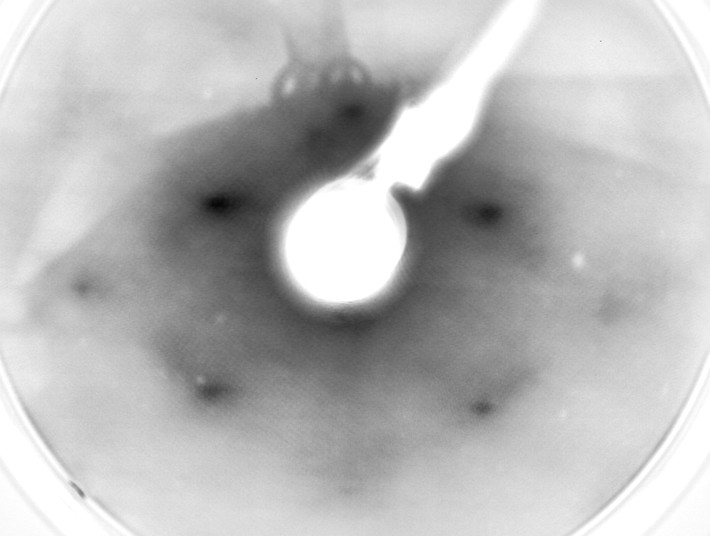
\includegraphics[width=\textwidth]{LEED-Bilder/bearbeitet/0_5ML_E208}
		\caption{\textit{1/2 Monolage Au}}
		\label{1/2ML} 
	\end{minipage}
	
	\begin{minipage}[b]{0.5\textwidth} 
		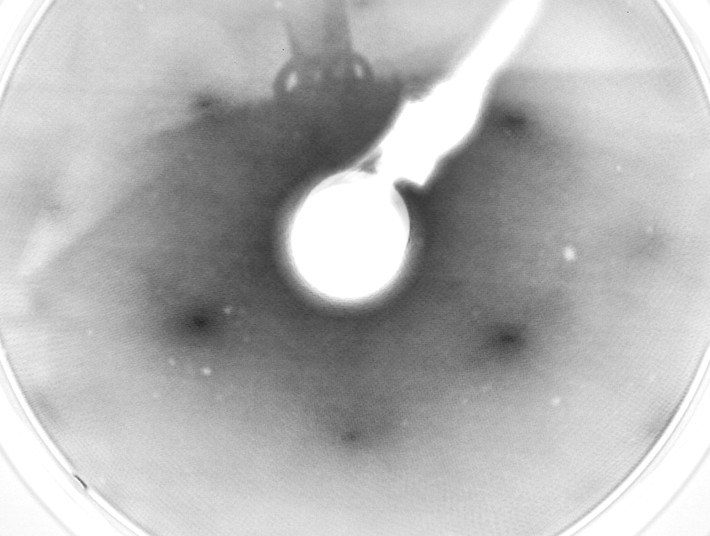
\includegraphics[width=\textwidth]{LEED-Bilder/bearbeitet/1ML_E207}
		\caption{\textit{1 Monolage Au}}
		\label{1ML} 
	\end{minipage}
	\hfill
	\begin{minipage}[b]{0.5\textwidth}
		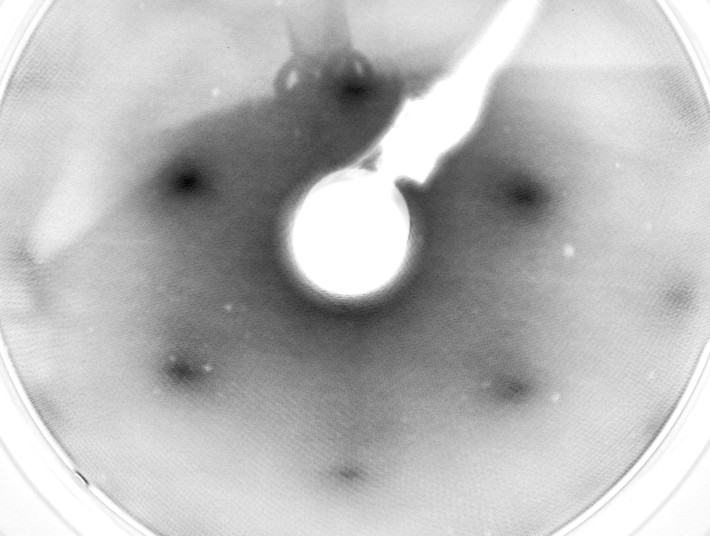
\includegraphics[width=\textwidth]{LEED-Bilder/bearbeitet/6ML_E207}
		\caption{\textit{6 Monolagen Au}}
		\label{6ML} 
	\end{minipage}
	
	\begin{minipage}[b]{0.5\textwidth} 
		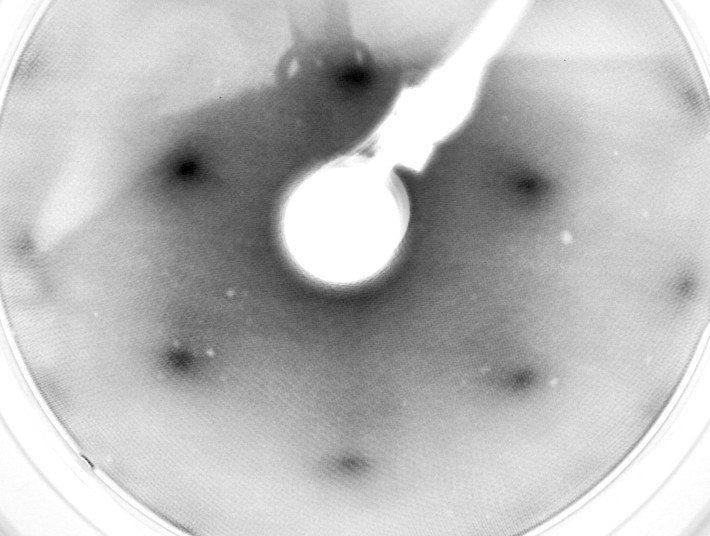
\includegraphics[width=\textwidth]{LEED-Bilder/bearbeitet/10ML_E207}
		\caption{\textit{10 Monolagen Au}}
		\label{10ML} 
	\end{minipage}
	\hfill
	\begin{minipage}[b]{0.5\textwidth}
		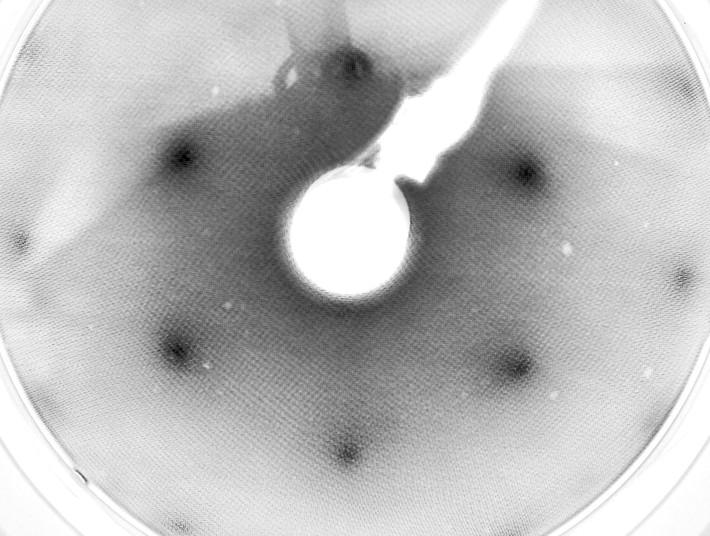
\includegraphics[width=\textwidth]{LEED-Bilder/bearbeitet/30ML_E208}
		\caption{\textit{30 Monolagen Au}}
		\label{30ML} 
	\end{minipage}
	\caption*{\textbf{Abb. 3.2-3.7:} \textit{LEED-Aufnahmen vom Re-Kristall ohne und mit
	verschiedenen Bedeckungsgraden von Gold bei einer Elektronenenergie von \SI{208}{eV}. In
	der Mitte ist die Elektronenkanone zu erkennen (weiß).}}
\end{figure}


Da zur Vermutung stand, diese Überstruktur könnte wie bei Wolfram von Kohlenstoffverunreinigungen
herrühren, wurde der Kristall unter einer Sauerstoffatmossphäre von etwa \SI{e-8}{mbar} bei einer
Temperatur von ungefähr \SI{1500}{K} geglüht. Dabei sollte der Kohlenstoff mit dem Sauerstoff zu
Kohlenmonoxid reagieren, welches durch Flashen von der Oberfläche entfernt werden kann. Dies
resultierte hier jedoch in keiner wesentlichen Verbesserung, sodass bei den folgenden LEED- sowie
STM-Messungen nur die äußeren Bereiche des Kristalls berücksichtigt wurden.
\\
Das Wachstum von Gold auf der Rheniumoberfläche wurde zuerst durch LEED für
verschiedene Bedeckungsgrade des Kristalls untersucht. Dazu wurden eine halbe, eine, sechs, zehn und
30 Monolagen auf den Kristall aufgedampft und die Beugungsmuster miteinander verglichen. Die
entstandenen Aufnahmen sind in den Abbildungen \ref{1/2ML} bis \ref{30ML} zu sehen, wie zum
Vergleich auch noch eine Abbildung der unbedampften Probenoberfläche. Alle Bilder entstanden
bei einer Elektronenenergie von \SI{208}{eV}.
\\
Zu erkennen ist eine deutliche Abschwächung der Intensität und eine Verbreiterung der Spots beim
Aufbringen einer halben Monolage Gold im Vergleich zum unbedampften Kristall. Auch bei anderen Energien des
Elektronenstrahls war kein deutlicheres Beugungsmuster zu erhalten; somit tragen viele der
gestreuten Strahlen zum Hintergrundleuchten bei, die Oberfläche besitzt also wenig Struktur.
Daraus lässt sich schließen, dass die aufgebrachten Goldatome kein pseudomorphes Wachstum betreiben, d.h.
sich nicht periodisch auf das Oberflächengitter des Substrats absetzen und dieses damit fortführen.
Die vorhandenden Spots stammen von der Substratoberfläche, an der tiefer eindringende Elektronen
gestreut werden. Bei einer aufgedampften Monolage verringert sich die Intensität der Spots noch
weiter; die Goldatome bilden offensichtlich bei dieser Schichtdicke noch keine erkennbare
Periodizität aus. Der Anteil der am Substrat gestreuten Elektronen wird allerdings geringer, da nun
die doppelte Anzahl von Goldatomen die Elektronen am tieferen Eindringen und Rückstreuen hindern.
\\
Ab sechs Monolagen Gold ist bis 30 Monolagen eine Steigerung der Intensität zu erkennen, die Spots
werden kleiner und schärfer. Das Gold bildet nun eine eigene periodische Struktur aus, die
Substratoberfläche trägt bei diesen Schichtdicken nur noch unwesentlich bzw. gar nicht mehr zum
Beugungsbild bei. Das Oberflächengitter der Adatome besitzt wiederum eine hexagonales Periodizität.
Obwohl Gold prinzipiell eine kubisch-flächenzentrierte Struktur besitzt, kann z.B. die (001)-Ebene
in einer hexagonalen Struktur rekonstruieren.
\\
Da höhere Anzahlen von Monolagen periodische Gitterstrukturen ausbilden und eine höhere
Oberflächengüte aufweisen, sind diese als Substrat für organische Moleküle besonders interessant.
Deren Anordnung und Struktur auf der Goldoberfläche lassen sich am besten auf großen, ebenen Flächen
untersuchen.
\\
Als nächstes wurden der unbedampfte Rheniumkristall sowie unterschiedliche Mengen Gold auf dessen
Oberfläche mittels STM untersucht. Dabei wurde der Konstantstrommodus mit einer Spannung von
\SI{0,6}{V} und einem Tunnelstrom von \SI{0,6}{nA} verwendet. In Abb. \ref{rekristallstm} sind zwei
verschieden große Ausschnitte der reinen Re-Oberfläche zu sehen. Gut zu erkennen sind etwa
\SI{35}{nm} breite Terassen mit einer Höhenvariabilität von ca. \SI{0,4}{nm}, was für eine plane,
regelmäßige Oberfläche spricht.
% Wie vielen Atomlagen entspricht das??
In der
Mitte des Kristalls wurden jedoch Fehlstellen wie in Abb. \ref{rekristallstm}b) gefunden.


\begin{figure}[htbp]
	\begin{minipage}[b]{0.5\textwidth} 
		\sffamily
		\includesvg[svgpath=goldaufre/]{rekristall1}
	\end{minipage}
	\hfill
	\begin{minipage}[b]{0.5\textwidth}
		\sffamily
		\includesvg[svgpath=goldaufre/]{rekristall2}
	\end{minipage}
	\caption{\textit{STM-Bilder der Rheniumoberfläche. a) Zu erkennen sind regelmäßig angeordnete
	Terrassen mit etwa 35nm Breite. b) In der Mitte der Probe sind auf dem Kristall Fehlstellen zu
	sehen (helle Streifen).}}
	\label{rekristallstm} 
	\begin{minipage}[b]{0.5\textwidth} 
		\sffamily
		\includesvg[svgpath=goldaufre/]{profilhalbeML}
	\end{minipage}
	\hfill
	\begin{minipage}[b]{0.5\textwidth}
		\sffamily
		\includesvg[svgpath=goldaufre/]{halbeML}
	\end{minipage}
	\caption{\textit{STM-Bilder von 0,5 Monolagen Gold auf Re. Es bilden sich Inseln aus
	mehreren Goldatomen von einer Größe von etwa \SI{7}{nm} Länge, die die Re-Oberfläche ungeordnet bedecken.}}
	\label{halbeML2stm} 
	\vfill
	\centering
	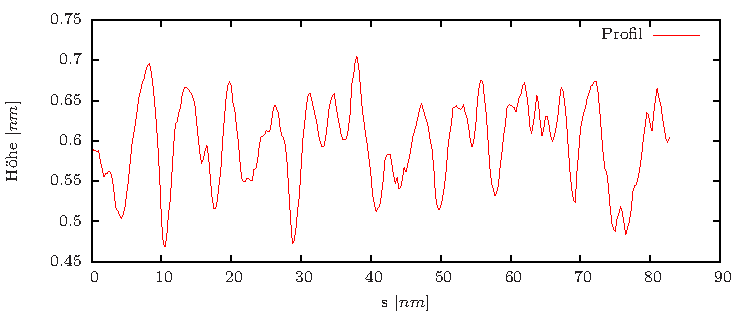
\includegraphics{pics/profilhalbeML}
	\caption{\textit{Höhenprofil aus Abb. \ref{halbeML2stm}a). Die Höhe der Goldinseln liegt bei etwa
	\SI{0,2}{nm}.}}
	\label{profilhalbeML} 
\end{figure}

% \begin{figure}[htbp]
% 	\centering
% 		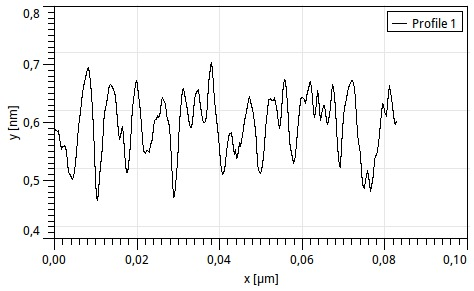
\includegraphics[height=6cm]{profilhalbeML.jpg}
% 	\caption{\textit{bla}}
% 	\label{profilhalbeML} 
% \end{figure}

\FloatBarrier

Betrachtet man eine halbe Monolage Gold auf der Oberfläche, ist ein Wachstum der Goldatome in
kleinen Inseln sehen, die die Substratoberfläche ungeordnet bedecken (Abb. \ref{halbeML2stm}).
Mit einem Höhenprofil wie in Abb. \ref{profilhalbeML} lässt sich eine Höhe der Inseln von
etwa \SI{0,2}{nm} bestimmen. Dies erklärt die schwache Intensität der Spots in der entsprechenden
LEED-Aufnahme, da die an den Goldatomen gestreuten Elektronen hauptsächlich zum Hintergrundleuchten
beitragen.
\\
Aus Zeitgründen wurde auf eine detailliertere Aufzeichnung des Lagenwachstums
verzichtet und stattdessen die als mögliche Substrate in Betracht kommenden Schichtdicken untersucht, in diesem
Fall 20 und 30 Monolagen Gold.\\
In Abb. \ref{MLVergleich} sind 20 und 30 Monolagen im Vergleich zu sehen. Es ist weiterhin ein
Inselwachstum zu beobachten.  Dabei beträgt die Höhendifferenz in beiden Bildern gleich bzw. weniger
als \SI{1,5}{nm}, was weniger als zehn Monolagen entspricht. Daraus kann man schließen, dass die
Monolagen unter den Inseln abgeschlossen sind. Solch ein Lagenwachstum, bei dem die nächste Lage beginnt zu
wachsen, ohne dass die darunter abgeschlossen ist, nennt man Stranski-Krastanov-Wachstum.


\begin{figure}[htbp]
	\begin{minipage}[b]{0.5\textwidth} 
		\sffamily
		\includesvg[svgpath=goldaufre/]{20ML}
	\end{minipage}
	\hfill
	\begin{minipage}[b]{0.5\textwidth}
		\sffamily
		\includesvg[svgpath=goldaufre/]{30ML}
	\end{minipage}
	\caption{\textit{STM-Bilder von a) 20 Monolagen Gold, b) 30 Monolagen Gold. Bei beiden
	Schichtdicken ist ein Inselwachstum zu beobachten mit einem Inseldurchmesser von etwa \SI{35}{nm}.}}
	\label{MLVergleich} 
\end{figure}

In beiden Fällen ist der Inseldurchmesser auf der abgeschlossenen Schicht etwa \SI{35}{nm}, der Durchmesser
der kleinsten, obersten Inseln etwa \SI{7}{nm}. Um das Wachstum aufgebrachter organischer Moleküle
auf Gold zu untersuchen, werden möglichst große, ebene Inseln benötigt. Durch die vielen Kanten ist dies bei
20 Monolagen nicht der Fall. Bei 30 Monolagen ergeben sich durchaus größere Inseln, die nicht durch
viele kleine Inseln bedeckt werden und damit als Molekülsubstrat brauchbar sind.\\
Ohne immer mehr Lagen aufdampfen zu müssen, um größere Inseln zu erhalten, kann man durch Tempern
oft ebenfalls eine Glättung der Oberfläche erreichen. Dabei wird durch Wärmestrahlung der Oberfläche
Energie zugeführt, bei der die Adatome nicht desorbieren, aber durch ihre erhöhte Mobilität
andere Strukturen aufbauen können. Hier wurden noch einmal 20 Monolagen Gold aufgedampft und zehn
Minuten mit einem Filamentstrom von \SI{2,0}{A} erhitzt (etwa \SI{650}{K}). Der Vergleich der
getemperten Probe zur ungetemperten ist in Abb. \ref{getVergleich} zu sehen.
Wie deutlich zu erkennen ist, verschwinden die kleinsten Inseln, es entstehen größere, flache
Inseln. Abb. \ref{profil20MLget} zeigt das Höhenprofil der in Abb. \ref{getVergleich}b)
eingezeichneten Linien. Die Inseln sind offensichtlich sehr eben: Die Oberfläche von Profil 1 ist
atomar glatt, während die von Profil 2 und 3 im Bereich von \SI{0,05}{nm} schwanken, was auch auf
Bildrauschen zurückzuführen sein kann. Die Größe und Flachheit der Inseln ist also durchaus als
Substrat für Moleküle geeignet. Falls erforderlich, könnten eventuell durch Tempern mit höherer
Temperatur eine weitere Glättung bzw. noch größere Inseln erreicht werden. 

\begin{figure}[htbp]
	\begin{minipage}[b]{0.5\textwidth} 
		\sffamily
		\includesvg[svgpath=goldaufre/]{20ML}
	\end{minipage}
	\hfill
	\begin{minipage}[b]{0.5\textwidth}
		\sffamily
		\includesvg[svgpath=goldaufre/]{20MLget2}
	\end{minipage}
	\caption{\textit{a) 20 Monolagen ungetempert, b) 20 Monolagen, 10 Minuten mit einem Filamentstrom
	von \SI{2,0}{A} getempert.
	Beim Tempern glättet sich die Oberfläche, es bilden sich größere, flache Inseln.}}
	\label{getVergleich} 
	\vfill
	\centering
		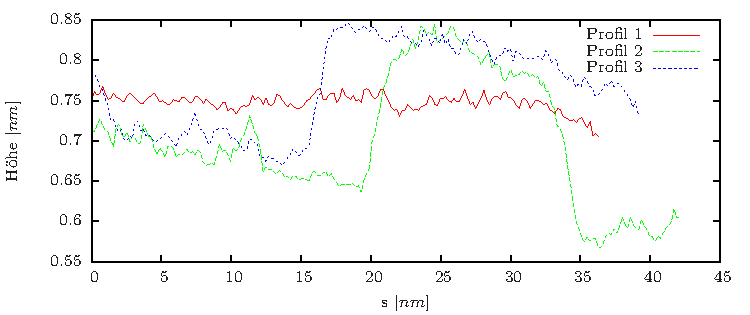
\includegraphics{pics/profiles20MLget}
	\caption{\textit{Höhenprofil aus Abb. \ref{getVergleich}b). Die Höhen der Oberflächen der Inseln
	schwanken im Bereich von etwa \SI{0,05}{nm}, somit sind die Inseln sehr eben.}}
	\label{profil20MLget}
\end{figure}